%************************************************
\chapter{Introduction}\label{ch:intro}
%************************************************
\section{Overview}
The efficient operation of railways depends upon the exchange of data, from passenger information such as timetables and delays, to operating data such as train locations, through to longer term planning operational data such as the projected cost of repairing equipment. Over time this data has been exchanged in different ways; from pioneering use of the telegraph for signalling, through to the large but siloed data stores we see today. As railway usage has increased\footnote{Passenger travel has risen 0.8\% year on year, see \autoref{state} and \citep{OfficeofRoad&Rail2016} for further details} and goals have been set to increase it further\footnote{For example the European Union transport white paper, \citet{EC2011} sets several long term goals for 2050 with the aim of reducing carbon, including \say{30\% of road freight over 300 km should shift to other modes such as rail or waterborne transport by 2030, and more than 50\% by 2050}.}, as a means of reducing the amount of carbon used by the economy, so more efficient data transfer is required. 

Presently systems are integrated on a costly system by system basis, for example using the Technical~Standards~for~Interoperability at points where the rail network crosses national boundaries within the European Union, or the Linear Asset Decision System for rail maintenance information within the UK. This means that most data generated are in proprietary formats and, as found by \citet{Kopf2010}, \say{most data are archived for \say{future use} and never looked at}. Poor data integration leads to increased costs, both directly incurred integrating systems and indirectly opportunities to save money or improve service are missed. Conversely if data is well integrated ridership (and hence income) can be increased with improved passenger information, maintenance costs can be lowered using predictive maintenance, more accurate cost projections can be made.

The need for improved integration has been recognised by the UK government which stated in the Rail Technical Strategy, a report by the \citet{TechnicalStrategyLeadershipGroup2012b}, it aspired to: ``[make] better use of the vast amounts of collected data''. The follow-up to the Rail Technical Strategy by the \citet{RDG2017}, which was reporting progress towards this goal, has a similar target: ``to share data effectively, asset owners need to establish data sharing principles and build a common architecture for sensor communication''.

Other studies, summarised in \autoref{sec:prevonto}, have examined the area of data integration in the rail domain and found ontology to be a useful tool. As a result several data models have been developed covering the rail domain, however, take up by industry remains limited. Given that the consensus of the literature (\citep{Kopf2010}, \citep{Gogos2016}, \citep{Verstichel2015} ) is that use of ontology will both save money and improve customer service, it seems paradoxical that take up remains very limited.  Improvements in customer information, the enabling of techniques such as predictive maintenance and the reduced ongoing cost of data integration are all made possible by using ontology for data integration. This thesis will investigate ways in which ontology could be more effectively used by industry.

%This prompts the question ``What is Ontology?'' . %Removed because it was a crap link
\subsection{What is ontology}

Ontology has different definitions dependant upon the field in which it is used. In philosophy the definition given by the Oxford English Dictionary: \say{the branch of metaphysics dealing with the nature of being} applies. This definition, whilst useful, differs somewhat from that used within computer science. In computer science ontologies are applied as a means of storing not just data, but information, that is data with meaning. In this domain the definition normally cited is:

\begin{quote}
An ontology is an explicit specification of a conceptualization. 
\end{quote}
\citet{gruber1993translation} 

 This definition alone requires further explanation, which is provided by the author, who defines a conceptualisation as: 
\begin{quote}
	The objects, concepts, and other entities that are presumed to exist in some area of interest and the relationships that hold them.
\end{quote}

 This use of ``Conceptualization'' is in turn taken from \citet{Genesereth1987}, who state that it offers an explicit view of the world. This is helpful in computer science because it allows software to work not just with data, but with knowledge. This knowledge in turn adds context to the information thus making information exchange easier.


Working with information, as opposed to data, is useful for integration, because once one stores the meaning of the data alongside the data itself it is much easier to integrate that data. Consider \autoref{fig:tab}; without any further context it is meaningless, just a list of nonsense words.

\begin{figure}[!htbp]
\myfloatalign
\fbox{{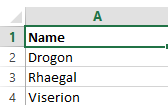
\includegraphics{gfx/dragonNames}} }
\caption{Tabular Data}
\label{fig:tab}
\end{figure}

 When however you consider \autoref{fig:ontoDragons} the meaning of the same data as shown in \autoref{fig:tab} becomes clear; it shows characters from a popular fantasy novel. 

\begin{figure}[!htbp]
\myfloatalign
\fbox{{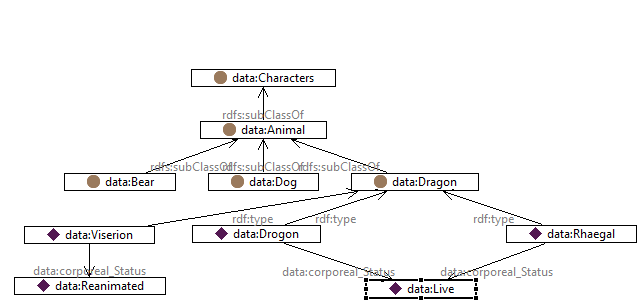
\includegraphics[width=\linewidth]{gfx/gameOfThronesDragons}} }
\caption{Ontology format}
\label{fig:ontoDragons}
\end{figure}

The intention is that by storing the meaning alongside the data it is straightforward, often not even requiring of human intervention, to combine that data with other data stored as information. Whilst this is true of any predefined schema the benefit of this approach is that it does not require such a central standards body to define a schema, instead any stakeholder can create data in this format, extending it to suit their needs, and still be able to integrate it with other data, allowing new data to be represented as and when it becomes available, without a lengthy approval process. 

\subsection{Barriers to adoption}
The fact that ontologies exist, and yet their adoption remains limited, implies that there are barriers to industry adoption of ontology. In the past technological maturity has been a serious obstacle; reasoning over large data stores is computationally expensive and neither robust software optimised for this task, nor hardware capable of running it has been available. Now the requisite hardware is available at a commodity price point and competing vendors for the relevant datastores exist in the marketplace so these barriers are eliminated. However a significant obstacle remains, in the form of a shortage of skilled personnel, ontology specialists and means of handling very high frequency data.

\section{Aims and Objectives}
This thesis will first investigate the current state of data integration in the rail domain, considering both solutions that employ ontology alongside more traditional techniques. The benefits of using ontology for data integration in the rail domain will then be assessed, taking into account progress made in other domains. This thesis will then examine the barriers to using ontology for data integration in the rail domain, before considering methods for overcoming those barriers. This thesis will then summarise tooling created to overcome the known barriers to adoption, and how these may be used within a typical industry workflow.

\section{Thesis organisation}
This document is organised as follows:

\begin{itemize}
	\item Chapter one is this introduction, which aims to set out the main themes of the thesis;
	\item Chapter two provides a review of the available literature on the topics covered by this thesis. In particular, the current situation with regards to data integration in the rail domain is examined, as are successful examples of data integration from other industries;
	\item Chapter three draws conclusions from the current situation out lined in chapter two and gives a more precise definition of the questions this thesis will answer;
	\item Chapter four investigates a typical industry data source and how it can be made available in a linked format;
	\item Chapter five investigates techniques for working with linked data, not requiring of skilled personnel;
	\item Chapter six investigates how multiple data sources can be brought together in an industry context;
	\item Chapter seven draws conclusions as to how data integration can be improved in the UK rail industry.
\end{itemize}

\section{Papers published over the course of this research}

The work presented in this thesis has been presented, in part, at a number of conferences.

\begin{itemize}	
	\item \textsc{Applications of Linked Data in the Rail Domain} \\ \textit{IEEE International Conference on Big Data 2014} \\
	This paper presents early findings from a larger study, into the use of linked data in the rail domain. The study and other literature has shown there to be benefits from improved integration of data in this domain and proposes that linked data in general and ontology in particular will address this. The paper will set out the current state of data integration in the British rail domain, highlighting issues found there. The manner in which linked data is employed in the broader transport domain will then be examined along with previous work pertaining to the rail domain. 
    \item \textsc{Ontology in the Rail Domain} \\ \textit{Knowledge Engineering and Ontology Development (KEOD) 2015} \\
    This paper presents the The Railway Core Ontologies (RaCoOn), a group of related ontologies designed to model the rail domain in detail. The purpose of these ontologies is to enable improved data integration in the rail domain, which will deliver business benefits in the form of improved customer perceptions and more efficient use of the rail network. The modularity of the ontologies allows for both detailed modelling of the domain at a high level and the storing of instance data at lower levels. It concludes that the benefits of improved rail data integration are best realised through the use of the railway core ontologies.   
    \item \textsc{FROM DATA TO INFORMATION: PROVISION OF RAILWAY DATA TO PASSENGERS IN THE INFORMATION AGE} \\ \textit{World Congress of Rail Research 2016} \\
    This paper puts forward the case for using RaCoOn for data integration in the the rail domain and sets out tools for expanding these ontologies.
\end{itemize}